% ------------------------------------------------------
\documentclass[pdftex,oneside,12pt,parskip=half,abstracton,ngerman]{scrartcl}
\usepackage{ngerman,a4}
\usepackage[english]{babel}
\usepackage[utf8]{inputenc}
\usepackage{a4wide}
\usepackage[printonlyused]{acronym}
\usepackage[automark]{scrpage2}
\automark{section}
\usepackage{pdfpages} 
\usepackage{listings}
\usepackage[scaled]{helvet}
\usepackage{courier}
\usepackage{color}
\usepackage{xcolor}
\usepackage{anysize}
\usepackage{amsmath}
\usepackage{amssymb}
\usepackage{textcomp}
\usepackage{geometry}
\geometry{
  left=1cm,
  right=1cm,
  top=1cm,
  bottom=1cm,
  bindingoffset=4mm
}
%Seitengroesse
\usepackage{fullpage}
%Zeilenumbruch und mehr
\usepackage[activate]{microtype}
% Zeilenabstand
\usepackage[onehalfspacing]{setspace}
\usepackage[babel,german=quotes]{csquotes}
\usepackage{framed}
% Spezielle Tabellenform fuer Deckblatt
\usepackage{longtable}
\setlength{\tabcolsep}{10pt} %Abstand zwischen Spalten
\renewcommand{\arraystretch}{1.0} %Zeilenabstand
\usepackage{pdfpages}
% ------------------------------------------------------
\begin{document}         
	% Start your text
% ------------------------------------------------------



% ------------------------------------------------------
% ------------------------------------------------------
% ------------------------------------------------------
\tableofcontents
\newpage
\section{Probeklausur}
\subsection{Erlaeutern sie kurz folgende Begriffe: Wiener Filter, Gauss Filter, Notch Filter und Histogram.}
\subsection{Aufgabe 2: Welche Verfahren verwendet man um weisses Rauschen zu unterdrücken?}
\subsection{Sie haben im Ortsbereich einen Spalttiefpass in Form einer 3 x 3 Matrix}
\subsection{Welcher der folgenden Filter ist ein Tiefpass?}
\subsection{Welcher Art sind die nachfolgenden Filter?
Falls mehrere Tiefpassfilter dabei sind, welcher hat den größten Weichzeichner?
Geben sie jeweils die Funktion für f(i, j) an.}
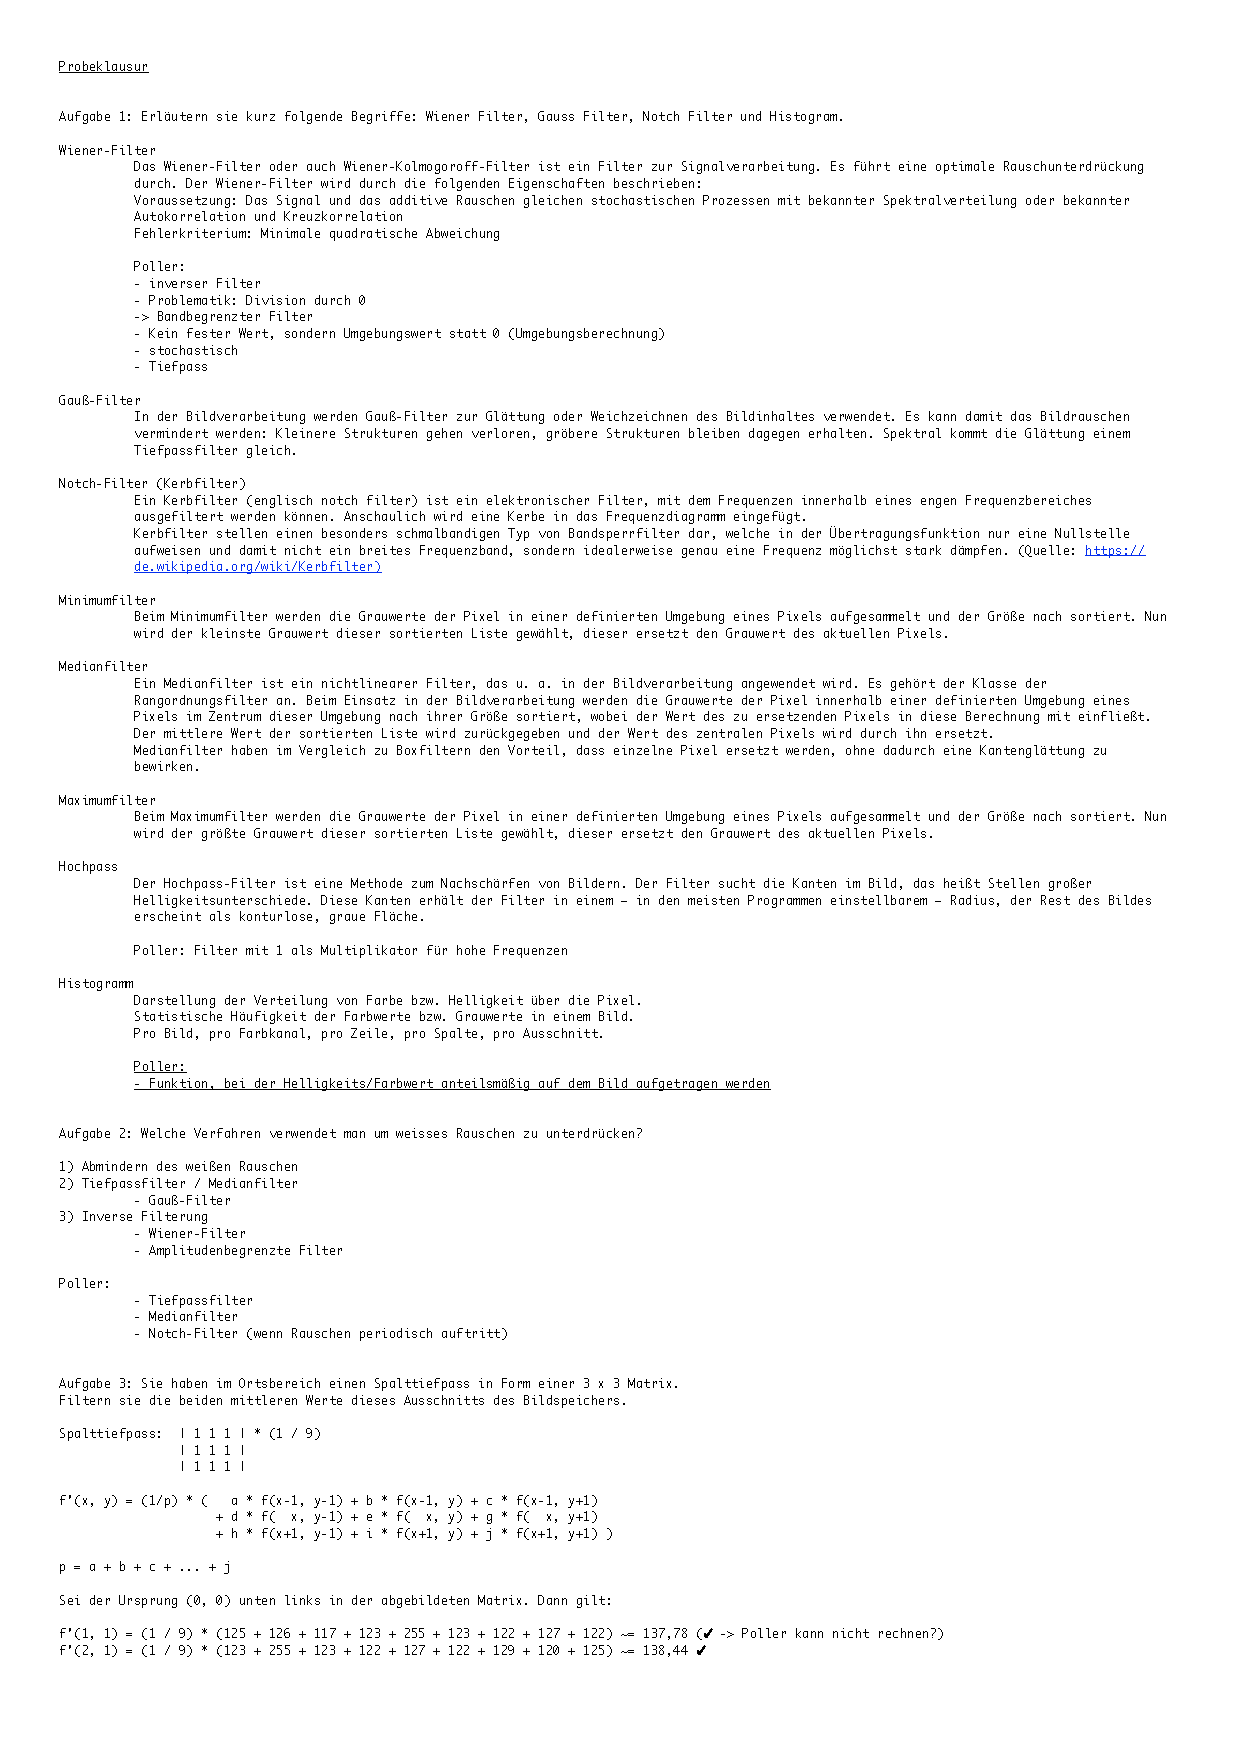
\includepdf[pages={1,2}]{input/neu.pdf}

% -------------------------------------------------------------------------_
% -------------------------------------------------------------------------_
% -------------------------------------------------------------------------_
\section{Hilfestellung zu genannten Aufgaben}
\subsection{Definition FFT,Hochpassfilter,Schwellwert}
\subsection{Tiefpass im Frequenzbereich und Ortsbereich beschreiben}
\subsection{Funktionsweise Inverser Filter}
\subsection{Rechenaufgaben wie in Probeklausur}
siehe oben :P
\subsection{KEINE Auswahl des geeignetsten Filters}

\section{Sonstige Informationen}
        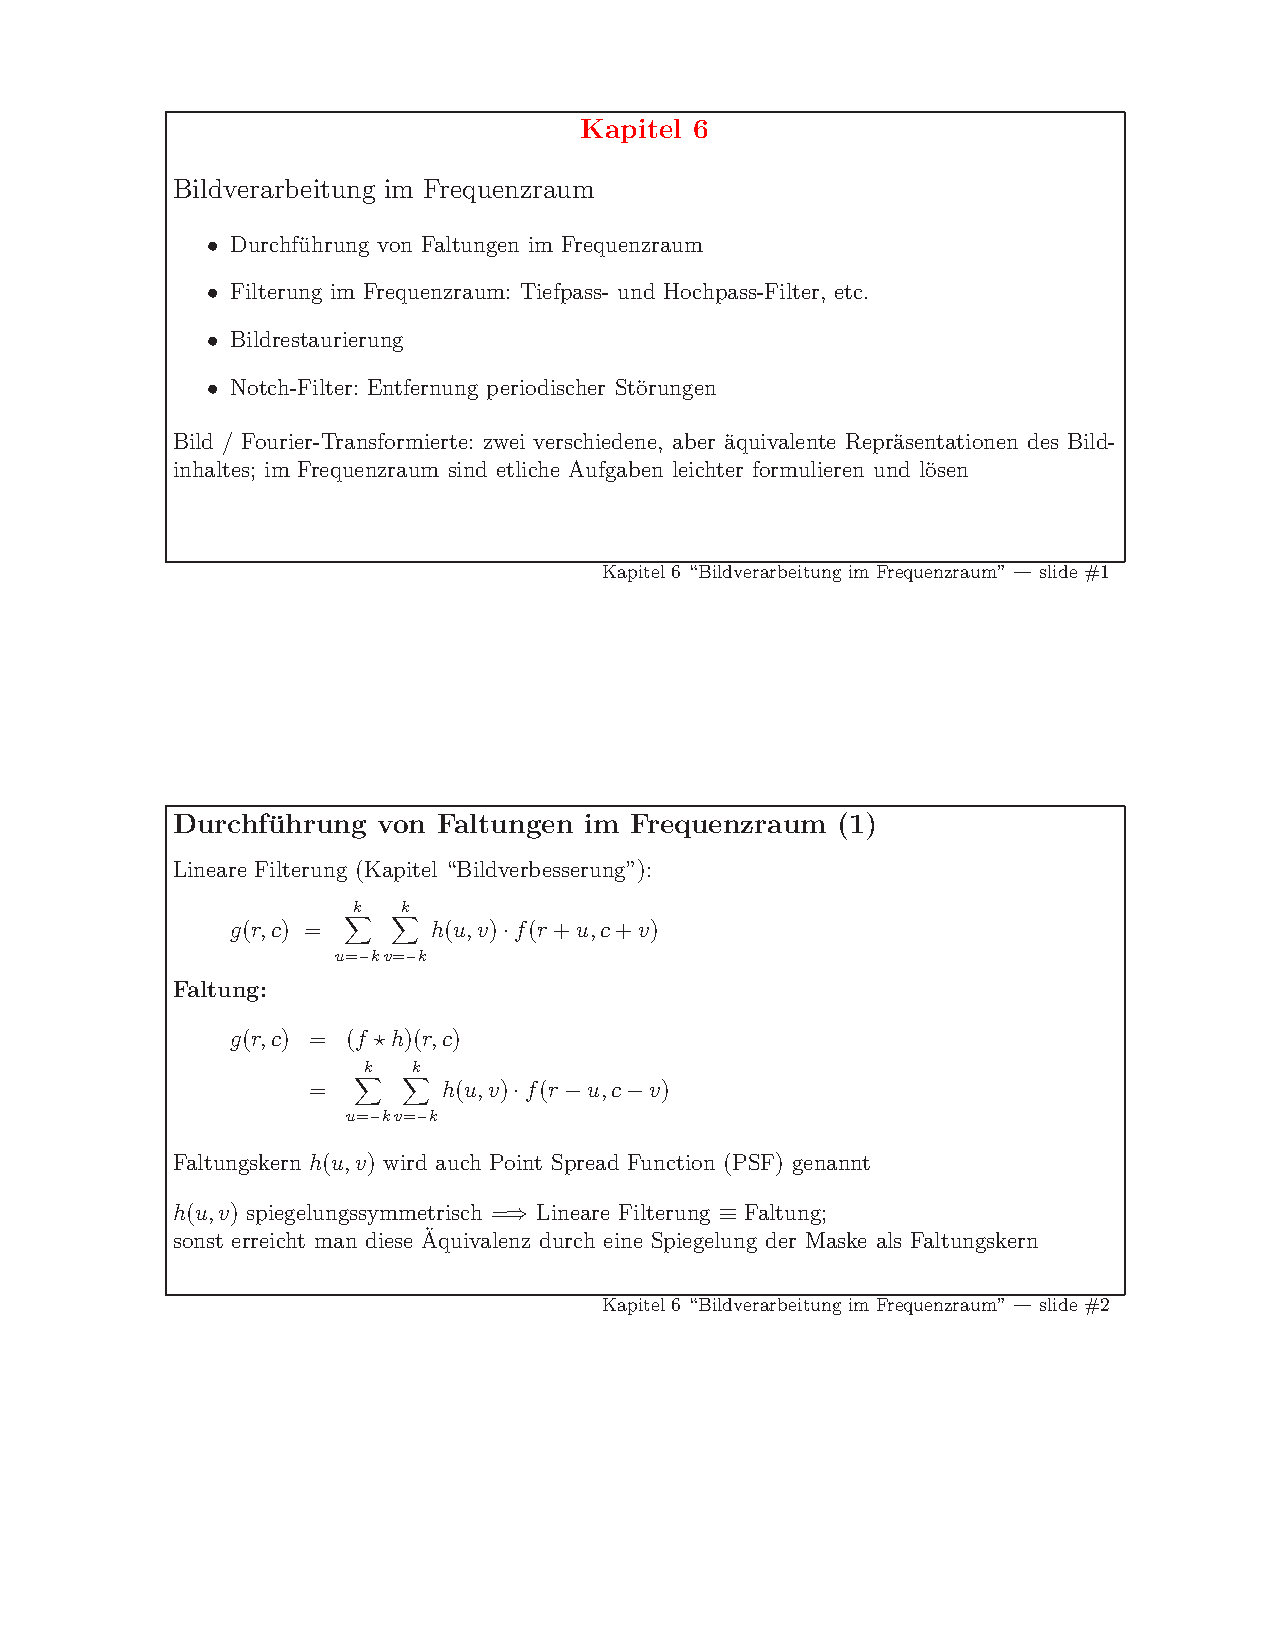
\includepdf[pages={1,4,5-8,13,15,16,17}]{input/1.pdf}
        \includepdf[pages={8,9,12,19,20}]{input/2.pdf}
        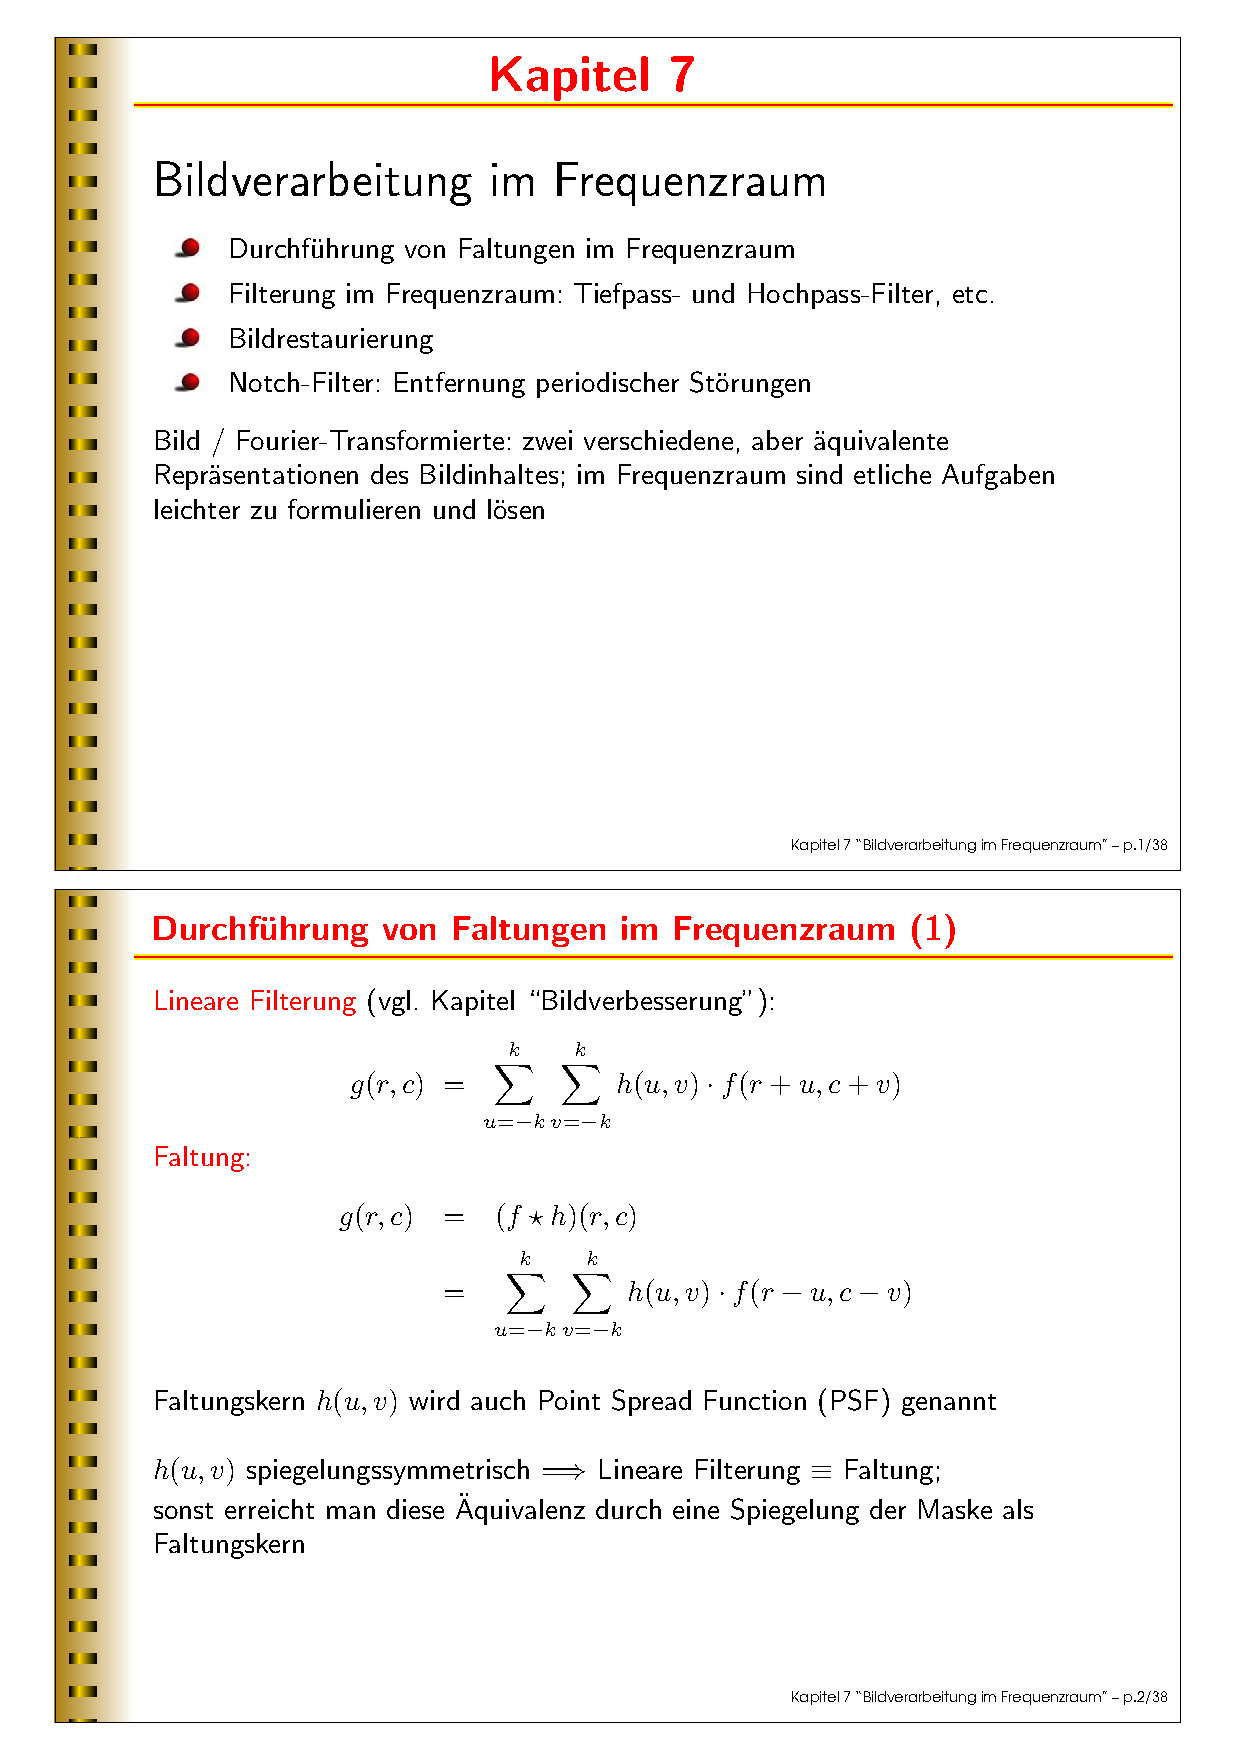
\includepdf[pages={1,4}]{input/3.pdf}
        \includepdf[pages={65,66}]{input/4.pdf}
% ------------------------------------------------------
% ------------------------------------------------------
% ------------------------------------------------------



% ------------------------------------------------------
	% Stop your text
\end{document}
% ------------------------------------------------------
